\section{Analysis on Weight Difference before and after COVID outbreak}

\

Here our goal is to check whether the COVID-situation had an impact on weight. We collected data from $230$ individuals and we have done the following study depending on that data.

\ 

Consider $(X_{1}, Y_{1})$, \ldots , $(X_{n}, Y_{n})$ being paired data of $n$-individuals, where :

$$X_{1}, \ldots , X_{n} \ \sim \ \text{IID} \ N(\mu, \sigma^{2}) \ : \ \text{weight distribution of $n$-individuals before COVID}$$
$$Y_{1}, \ldots , Y_{n} \ \sim \ \text{IID} \ N(\mu, \sigma^{2}) \ : \ \text{weight distribution of $n$-individuals after COVID}$$

Here, 
$$E(X_{i}) \ = \ \mu_{1} , \ V(X_{i}) \ = \ \sigma_{1}^{2} , \ \forall \ i \ = \ 1, 2, \ \ldots \ , n$$
$$E(Y_{i}) \ = \ \mu_{2} , \ V(Y_{i}) \ = \ \sigma_{2}^{2} , \ \forall \ i \ = \ 1, 2, \ \ldots \ , n$$
where $\sigma_{1}, \sigma_{2}$ are unknowns.

\ 

Assuming normality, we will assess whether the weights remain the same before and after COVID, testing against the alternative hypothesis that they do not.

\ 

\textbf{Hypothesis}:
$$H_{0} \ : \ \mu_{1} \ = \ \mu_{2} \ \text{  vs  } \ H_{1} \ : \ \mu_{1} \ \neq \ \mu_{2}$$

\ 

Here, $(X_{i}, Y_{i}) \ \sim \ \text{BVN} \ (\mu_{1}, \ \mu_{2}, \ \sigma_{1}^{2}, \ \sigma_{2}^{2}, \ \rho)$, where $\rho$ being the correlation coefficient of $X_{i}$ and $Y_{i}$.

\ 

So Let's take, 
$$D_{i} \ = \ X_{i} \ - \ Y_{i}, \ \forall \ i \ = \ 1, 2, ... \ , n$$
$$D_{1}, \ \ldots \ , D_{n} \ \text{are IID} \ N(\mu_{1} - \mu_{2}, \ \sigma^{2}), \text{ where } \ \sigma^{2} \ \text{unknown}.$$

\newpage

where we have,
$$\sigma^{2} \ = \ V(X) \ + \ V(Y) \ - \ 2 \cdot \text{Cov} (X, Y)$$
$$= \ \sigma_{1}^{2} \ + \ \sigma_{2}^{2} \ - \ 2 \cdot \rho \cdot \sigma_{1} \cdot \sigma_{2}$$

\ 

Now, the above test becomes equivalent to one sample test of
$$H_{0} \ : \ \mu \ = \ 0 \ \text{  vs  } \ H_{1} \ : \ \mu \ \neq \ 0 \ \text{with unknown} \ \sigma^{2}$$
where, \ $\mu \ = \ \mu_{1} \ - \ \mu_{2}$.

\

 In this two-tailed test, consider
 $$\Bar{D} \ = \ \frac{D_{1} \ + \ \ldots \ + \ D_{n}}{n}$$
 \[E\left[\Bar{D}\right] = E\left[\frac{D_{1} + \ldots + D_{n}}{n}\right] = \frac{n\cdot\mu}{n} = \mu\]
 \[V\left[\Bar{D}\right] = V\left[\frac{D_{1} + \ldots + D_{n}}{n}\right] = \frac{1}{n^{2}} \left\{ V[D_{1}] + \ldots + V[D_{n}] \right\}\]
 \[= \frac{1}{n^{2}} \ n\sigma^{2} = \frac{\sigma^{2}}{n}, \quad \text{as $D_{1}, \ \ldots \ , D_{n}$ are IID}\]

 \ 

thus, $\Bar{D} \sim N(\mu, \frac{\sigma^{2}}{n})$.

 \ 

\textbf{Test Statistics}:
Consider following test-statistic using paired \textit{$t-test$}.
$$T \ = \ \frac{\Bar{D} \ - \ \mu}{\frac{s}{\sqrt{n}}} , \ \ \text{where $s$ being sample standard-deviation}$$

and $T \ \sim \ t_{n-1}$, i.e. $t$-distribution with $(n-1)$ degrees of freedom.

\ 

Now, based on our data collected form $n \ = \ 230$ observations : 
\begin{center}
    \fbox{\parbox{\textwidth}{
$$\text{Sample Mean} \ = \ \Bar{d} \ = \ 3.058696$$
$$\text{Sample Median} \ = \ m_{e} \ = \ 3$$
$$\text{Sample Variance} \ = \ 45.643920$$
$$\text{Sample Standard deviation} \ = \ 6.756028$$
}}
\end{center}


\newpage 

Now, under the null-hypothesis $\mu \ = \ 0$ and $s \ = \ 0$,
$$T \ = \ \frac{\Bar{D} \cdot \sqrt{n}}{s}$$

using the above data,
$$t \ \approx \ 6.866079, \ \text{observed value of} \ T.$$

\ 

\textbf{Critical Region} :
Since, $n \ = \ 230$ and $d.f.$ \ $= \ 229$, then
$$T \ \sim \ t_{229, \ 0.975}$$
thus critical region at $5\%$ level of significance is
$$(-\infty , \ 1.9709] \ \bigcup \ [1.9709, \ \infty).$$

\ 

\textbf{Decision Rule}: To make our decision, we will check if test-statistics lies in confidence interval or not. Our test-statistic is $t \ = \ 6.866079$.

\

If $t$ lies within the critical region, we reject null-hypothesis.

\ 

\textbf{Decision}: Since, 
$$t \ = \ 6.866079 \ > \ t_{229, \ 0.975} \ = \ 1.9709$$
i.e. $t$ lies within the critical region $(-\infty , \ 1.9709] \ \cup \ [1.9709, \ \infty)$. 

\

Therefore, we \textbf{reject null hypothesis} $H_{0} \ : \ \mu \ = \ 0$ against $H_{1} \ : \ \mu \ \neq \ 0$.

\begin{figure}[h!]
	\centering
	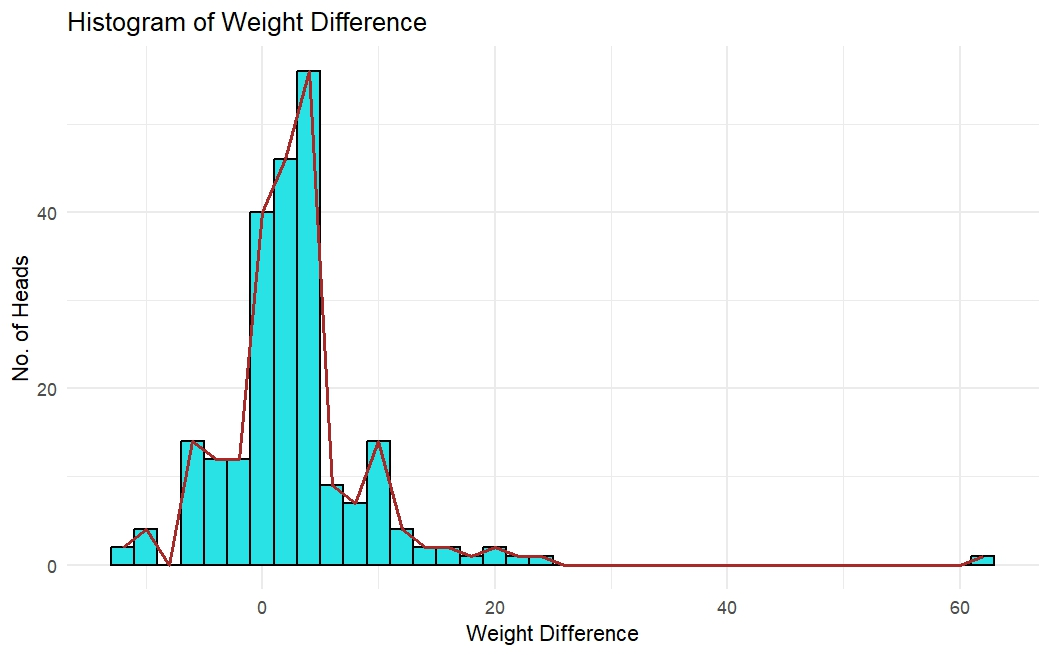
\includegraphics[width=0.7\linewidth]{IMAGES/Image 39.jpg}
	\caption{Difference in Weights}
	\label{G39}
\end{figure}

Above, in Figure \ref{G39} we provide a pictorial representation of our data set of weight difference

\

\textbf{Result Interpretation}: Rejecting null-hypothesis provides strong evidence that there is a statistically significant difference in weights before and after COVID-19.

\ 

Hence, our study shows COVID-19 pandemic might had an impact on individual's weight.
 
\ 

We have outliers in our data set. Except these, our data set is clustered between $-20$ to $30$, which indicates persons under study may have encountered significant changes in their weights.

\ 

From the graph above shown (figure \ref{G39}), indicates the mean is greater than zero, which means there is a high probability that individual's had his/her weight decreased after COVID-situation.
